\section{harps::Clock$<$ \_\-sampling\_\-rate, \_\-sample\_\-count $>$ Class Template Reference}
\label{classharps_1_1Clock}\index{harps::Clock@{harps::Clock}}
{\tt \#include $<$clock.hpp$>$}

Inheritance diagram for harps::Clock$<$ \_\-sampling\_\-rate, \_\-sample\_\-count $>$::\begin{figure}[H]
\begin{center}
\leavevmode
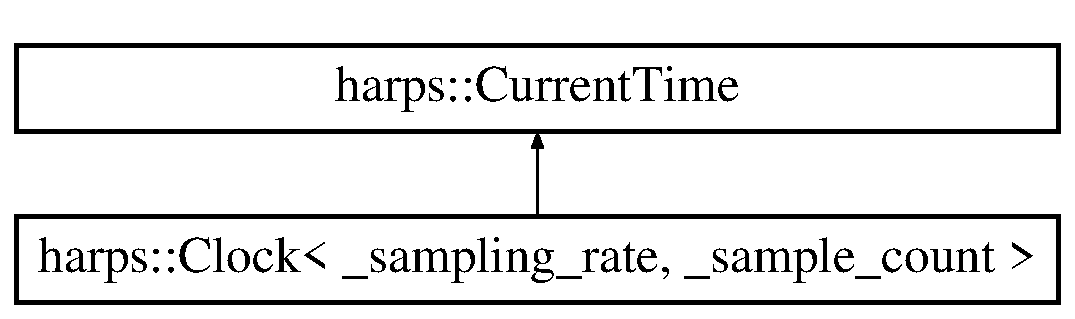
\includegraphics[height=2cm]{classharps_1_1Clock}
\end{center}
\end{figure}
\subsection*{Public Member Functions}
\begin{CompactItemize}
\item 
void \textbf{tick} ()\label{classharps_1_1Clock_39971acf3b3d864c1e3484ee055d93ef}

\end{CompactItemize}


\subsection{Detailed Description}
\subsubsection*{template$<$unsigned int \_\-sampling\_\-rate, unsigned int \_\-sample\_\-count$>$ class harps::Clock$<$ \_\-sampling\_\-rate, \_\-sample\_\-count $>$}

CurrentTimeのtick幅をバッファの長さに固定したものです。 

The documentation for this class was generated from the following file:\begin{CompactItemize}
\item 
rc/harps/include/harps/clock.hpp\end{CompactItemize}
